

\actTitle{Worksheet 4.2B}



\noindent \textbf{Instructions:}  Work together in groups of  3 or 4 to complete the following problems.\\


\begin{enumerate}


\item The coordinate $P\left(5/6,-\sqrt{11}/6)\right)$ is on the unit circle and corresponds to
  the real number $t$.

\begin{enumerate}
\item Make a diagram of the unit circle with $P$ on it. Indicate the
  angle $t$ and annotate the point, $P$.

  \vfill
  \vfill

\item Determine the values of the six trig functions at $t$. 

\begin{tabular}{l@{\hspace{0.25\textwidth}}l@{\hspace{0.25\textwidth}}l@{\hspace{0.25\textwidth}} }
$\sin(t)=$ &  $\cos(t)=$ & $\tan(t)=$    \\
& & \\
& & \\
$\csc(t)=$ &  $\sec(t)=$   & $\cot(t)=$    \\
& & \\

\end{tabular}\\


\item Determine $\cos(-t)$ and $\sin(-t)$ including a brief
  justification using the unit circle you drew above.

  \vfill

\item Determine $\sin(t+2\pi)$ and $\cos(t+2\pi)$ including a brief
  justification using the unit circle you drew above.

  \vfill

\end{enumerate}

\clearpage

\item $P(x,y) = \left(\frac{4}{5}, \frac{3}{5}\right)$ corresponds to a real number $t$. 
\begin{enumerate}
\item Make a diagram of the unit circle with $P$ on it.

  \vfill

\item Determine $\cos(t)$ and $\sin(t)$.

  \vfill

\item Determine $\cos(t+4\pi)$ and $\sin(t-6\pi)$.

  \vfill

\item Determine $\cos(-t)$ and $\sin(-t)$. Use your drawing above to
  provide a brief justification of your result.

  \vfill

\item Determine $\cos(-t-4\pi)$ and $\sin(-t+100\pi)$. Provide a brief
  justification of your result.

  \vfill
  
\end{enumerate}


\clearpage

\item Given $\cot(t)=\frac{45}{28}$ for $\pi<t<\frac{3\pi}{2}$.  Use
  an appropriate Pythagorean identity to find the value of $\csc(t)$
  (Provide a rough sketch of the situation and use your sketch to
  provide a quick justification for the important decisions you have
  to make.)

  \vfill
  
\item Write $\tan(t)$ in terms of $\sec(t)$ for
  \sideNote{Include a rough sketch of the situation in each case.}
\begin{enumerate}
\begin{multicols}{2}
\item $t$ in Quadrant 2.

\columnbreak
\item $t$ in Quadrant 4.
\end{multicols}
\end{enumerate}

\vfill

\clearpage

\item Use the periodic properties of the trigonometric functions to simplify each expression to a \textbf{single} function of $t$.

\begin{enumerate} 
\item $\sin(t+2\pi)\cdot \cot(t+\pi)$\vfill
\item  $\sin(t+2\pi)\cdot \sec(t+2\pi)$\vfill
\end{enumerate}



\item Use the even-odd and periodic properties of the trigonometric functions to simplify.
\begin{enumerate}
\item $\csc(t)-4\csc(-t)$\vfill
\item $-2\sin(3t+2\pi)-3\sin(-3t)$\vfill
\end{enumerate}

\vfill


\item Simplify using properties of trigonometric functions. $$\sin^2(t+2\pi)+\cos^2(t)+\tan^2(t+\pi)$$
\vfill

\clearpage
\item Identify values $t$ on the interval $[0,2\pi]$ that make the given function undefined (if any).
\begin{enumerate}
\begin{multicols}{2}
\item $y=\sin(t)$\\[.3in]
\item $y=\cot(t)$\\[.3in]
\item $y=\cos(t)$\\[.3in]
\columnbreak
\item $y=\tan(t)$\\[.3in]
\item $y=\csc(t)$\\[.3in]
\item $y=\sec(t)$\\[.3in]
\end{multicols}
\end{enumerate}

\item Write down all trig functions for which each property applies.
\begin{enumerate}
\item The function is even.\vfill
\item The function is odd.\vfill
\item The period is $2\pi$.\vfill
\item The period is $\pi$.\vfill
\item The domain is all real numbers.\vfill
\item The domain is all real numbers excluding odd multiples of $\frac{\pi}{2}$.\vfill
\item The domain is all real numbers excluding multiples of $\pi$.\vfill
\end{enumerate}

\end{enumerate}

\hwTitle{Section 4.2B}

\begin{enumerate}


\item If you plan on using the unit circle instead of special
  triangles and the chart for angles on the $x$ and $y$ axes, start
  memorizing the angles of the unit circle in radians as well as the
  points along the unit circle.


\noindent
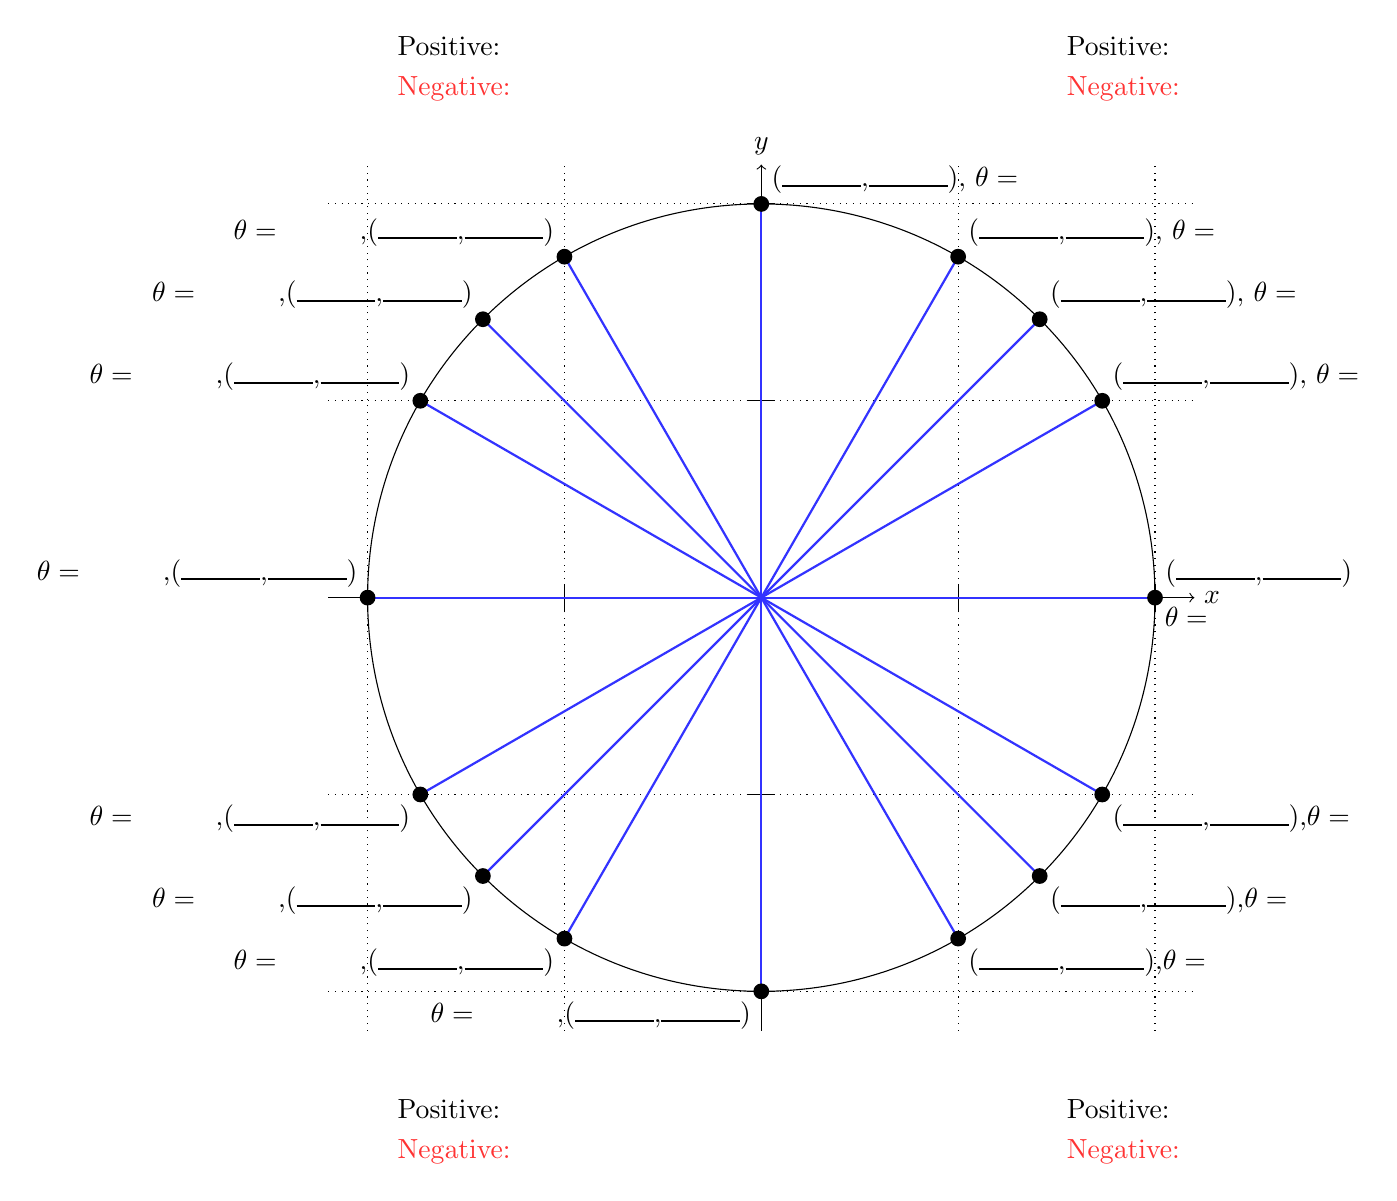
\begin{tikzpicture}[scale=5]
  \draw[step=0.5cm,black, dotted] (-1.1,-1.1) grid (1.1,1.1); % very thin,
  \draw[->] (-1.1,0) -- (1.1,0) node[anchor=west] {$x$};
  \draw[->] (0,-1.1) -- (0,1.1) node[anchor=south] {$y$};
  \draw (0,0) circle(1);

  \foreach \x in {-1,-0.5,0.5,1} {
    \draw (\x cm,1pt) -- (\x cm,-1pt);
    %%\draw (\x cm,-1pt) node[anchor=north,fill=white] {$\x$};
  }

  \foreach \y in {-1,-0.5,0.5,1}{
    \draw (-1pt,\y cm) -- (1pt,\y cm);
    %%\draw (-1pt,\y cm) node[anchor=east,fill=white] {$\y$};
  }
  
  %\draw[green,thick] (.2cm,0cm) arc [start angle=0, end angle=0,radius=.2cm];
  \draw[blue!80,thick] (0,0) -- (0:1)
     node[black,anchor=south west] {(\rule{1cm}{0.025cm},\rule{1cm}{0.025cm})};
  \node[black,anchor=north west] at (0:1) {$\theta=$};
  \fill[black] (0:1) circle (0.02);

  \foreach \y in {30,45,60,90}{
    \draw[blue!80,thick] (0,0) -- (\y:1)
        node[black,anchor=south west] {(\rule{1cm}{0.025cm},\rule{1cm}{0.025cm}), $\theta=$};
    \fill[black] (\y:1) circle (0.02);
  }
  \foreach \y in {120,135,150,180}{
    \draw[blue!80,thick] (0,0) -- (\y:1)
        node[black,anchor=south east] {$\theta=$~~~~~~~~~,(\rule{1cm}{0.025cm},\rule{1cm}{0.025cm})};
    \fill[black] (\y:1) circle (0.02);
  }
  \foreach \y in {210,225,240,270}{
    \draw[blue!80,thick] (0,0) -- (\y:1)
        node[black,anchor=north east] {$\theta=$~~~~~~~~~,(\rule{1cm}{0.025cm},\rule{1cm}{0.025cm})};
    \fill[black] (\y:1) circle (0.02);
  }
  \foreach \y in {300,315,330}{
    \draw[blue!80,thick] (0,0) -- (\y:1)
        node[black,anchor=north west] {(\rule{1cm}{0.025cm},\rule{1cm}{0.025cm}),$\theta=$};
    \fill[black] (\y:1) circle (0.02);
  }


  \foreach \x in {0.75,-0.95} {
    \foreach \y in {-1.35,1.35} {
      \node[black,thick,anchor=south west]  at (\x,\y) {Positive:};
      \node[red!80,thick,anchor=north west] at (\x,\y) {Negative:};
    }
  }
\end{tikzpicture}

\item Each of the following questions refer to points on the edge of a
  circle that is centered at the origin.
  \begin{enumerate}
  \item A point on a circle of radius four is in the second
    quadrant. The point is given by $P(-2.7, y)$. Determine the cosine
    and sine of the angle formed by the ray to $P$ and the positive
    $x$-axis.
  \item A point on a circle of radius two is in the third
    quadrant. The point is given by $P(x, -1.2)$. Determine the cosine
    and sine of the angle formed by the ray to $P$ and the positive
    $x$-axis.
  \item What are coordinates (The x and y values) of the point on the
    unit circle where the angle between the ray through the point and
    the positive x-axis is $\frac{11\pi}{6}$ radians?
  \item The point $P$ is in the first quadrant. What are the possible
    range of values for the sine of the angle formed by the ray to $P$
    and the positive $x$-axis? What are the possible range of values
    for the cosine of the angle?
  \item The point $P$ is in the fourth quadrant. What are the possible
    range of values for the sine of the angle formed by the ray to $P$
    and the positive $x$-axis? What are the possible range of values
    for the cosine of the angle?
  \end{enumerate}

\item The radian measure of the angle $\alpha$ satisfies
  $\frac{\pi}{2}<\alpha<\pi$. The radian measure of the angle $\beta$
  satisfies $\frac{3\pi}{2}<\beta<2\pi$.  Given the values below
  determine the values of each of the quantities below:
  \begin{eqnarray*}
    \sin(\alpha) & = & \frac{5}{9}, \\
    \cos(\beta)  & = & \frac{2}{7}.
  \end{eqnarray*}
  
  \begin{enumerate}
    \begin{multicols}{2}
    \item ${\displaystyle \cos(\alpha) }$
    \item ${\displaystyle \sin(-\alpha) }$
    \item ${\displaystyle \sin(\pi+\alpha) }$
      \columnbreak
    \item ${\displaystyle \sin(\pi+\beta) }$
    \item ${\displaystyle \cos(\alpha-\pi) }$
    \item ${\displaystyle \tan(\alpha+\pi)\cdot\tan(\beta-\pi) }$
    \end{multicols}
  \end{enumerate}

\item Determine the values of the cosine and sine of the angles
  indicated in each of the following questions.

  \begin{enumerate}
  \item The point shown in the diagram below is on the \textbf{unit
      circle}.  Determine the values of the cosine, sine, and tangent
    of the angle $\delta$ as shown in the diagram.
    

    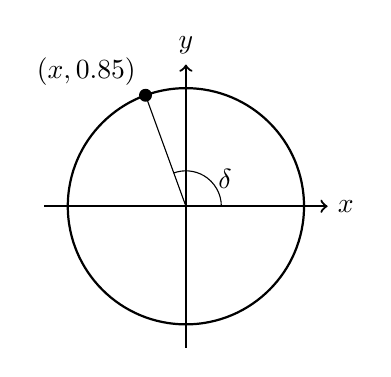
\begin{tikzpicture}[y=1.5cm, x=1.5cm,font=\sffamily]
      \draw[thick,black,->] (-1.2,0) -- (1.2,0) node[anchor=west] {$x$};
      \draw[thick,black,->] (0,-1.2) -- (0,1.2) node[anchor=south] {$y$};
      \draw[thick,black] (0,0) circle (1);
      \draw[black,fill=black] (0,0) -- (110:1) circle (0.05) node[anchor=south east] {$(x,0.85)$}  ; % ,fill=gray
      \node[black,anchor=west] at (50:0.3)  {$\delta$};
      \draw[thin,black] (0:0.3) arc (0:110:0.3);
    \end{tikzpicture}

  \item The point shown in the diagram below is on the \textbf{unit
      circle}.  Determine the values of the cosine, sine, and tangent
    of the angle $\gamma$ as shown in the diagram.
    

    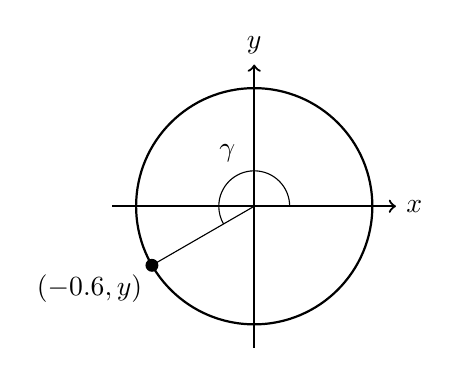
\begin{tikzpicture}[y=1.5cm, x=1.5cm,font=\sffamily]
      \draw[thick,black,->] (-1.2,0) -- (1.2,0) node[anchor=west] {$x$};
      \draw[thick,black,->] (0,-1.2) -- (0,1.2) node[anchor=south] {$y$};
      \draw[thick,black] (0,0) circle (1);
      \draw[black,fill=black] (0,0) -- (210:1) circle (0.05) node[anchor=north east] {$(-0.6,y)$}  ; % ,fill=gray
      %\node[black,anchor=west] at (50:0.3)  {$\delta$};
      \draw[thin,black] (0:0.3) arc (0:210:0.3) node[pos=0.5,anchor=south east] {$\gamma$};
    \end{tikzpicture}

  \end{enumerate}


\end{enumerate}
